\chapter{Circular Motion}
\begin{figure}[H]
    \centering
    \includegraphics[page=5]{../images/Circular-motion-image/Circular-motion-image.pdf}
    \caption{\ref{source:circular-motion-thumbnail} An illustration of circular motion.}
    \label{fig:circular-motion-thumbnail}
\end{figure}
\begin{itemize}
    \item \emph{Angular displacement} is the angle through which an object turns \emph{with respect to the center} of its circular path.
    \item \emph{The radian} is defined as the angle \emph{subtended} at the \emph{center} of a circle by an \emph{arc} of length equal to the radius of the circle. 
    \item \emph{Angular velocity} is the rate of change of angular displacement.
\end{itemize}
\begin{itemize}[label=\(\square\)]
    \item \begin{tabular}{|Sc|Sc|Sc|Sc|Sc|}
        \hline
            \(\begin{aligned}
                \omega=\frac{2\pi}{T}=2\pi f
            \end{aligned}\)&
            \(\begin{aligned}
                v=r\omega
            \end{aligned}\)&
            \(\begin{aligned}
                a_c=\frac{v^2}{r}=r\omega^2=v\omega
            \end{aligned}\)&
            \(\begin{aligned}
                F_c=ma_c
            \end{aligned}\)
        \\
        \hline
    \end{tabular}
    \item Common formulae: \(\tan(\theta)=\left(\frac{v^2}{rg}\right)\) and \(v=\sqrt{rg}\).
    \begin{figure}[H]
        \centering
        \begin{subfigure}[c]{0.55\textwidth}
            \centering
            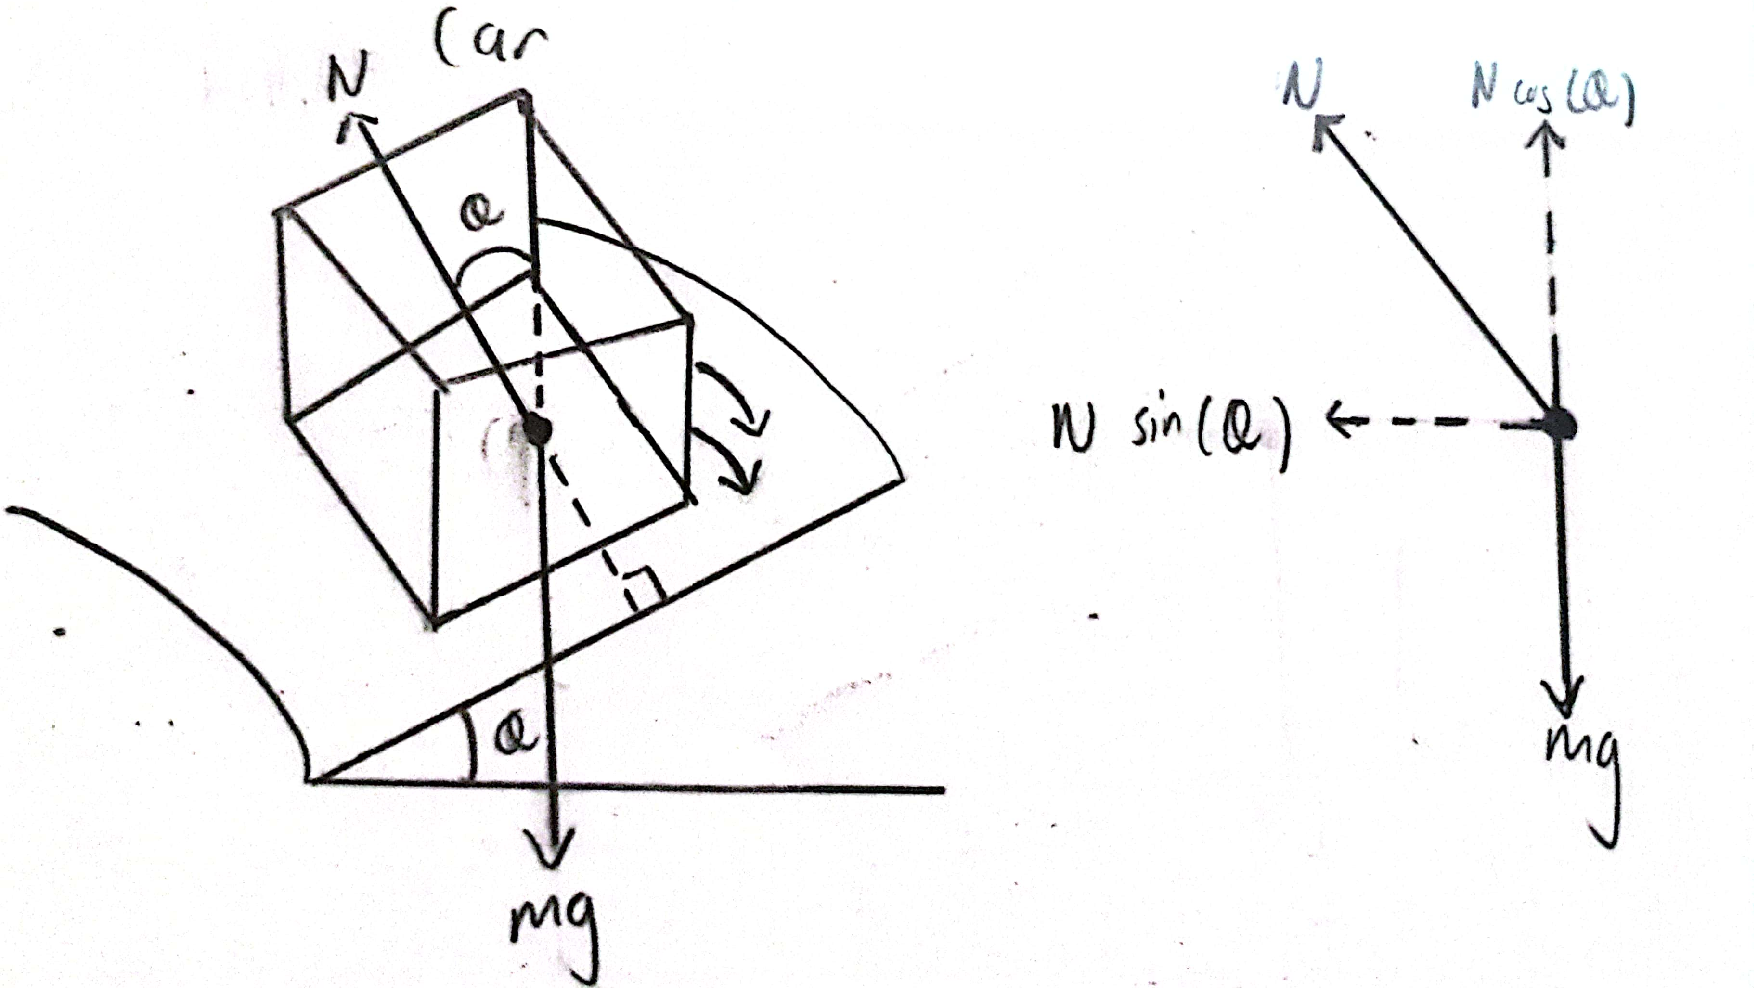
\includegraphics[width=\textwidth,page=1]{../images/Circular-motion-examples.pdf}
            \caption{\(\tan(\theta)=\frac{v^2}{rg}\)}
        \end{subfigure}%
        \hfill
        \begin{subfigure}[c]{0.35\textwidth}
            \centering
            \vspace{0.5cm}
            \includegraphics[width=\textwidth,page=2]{../images/Circular-motion-examples.pdf}
            \vspace{0.5cm}
            \caption{\(v=\sqrt{rg}\)}
        \end{subfigure}%
        \caption{\ref{Me} Example situations where we will use \(\tan(\theta)=\frac{v^2}{rg}\) and \(v=\sqrt{rg}\).}
        \label{table:circular-motion-examples}
    \end{figure}
    \item Water in bucket at top position: \(F_c=N+W\) (where \(N\geq 0\)) so \(\omega\geq\sqrt{\frac{g}{r}}\).
    \item We need to write ``Centripetal force is provided by \underline{\hspace{1cm}}'' 
    \item Why are teardrop designs preferred over full circles for roller coaster tracks? It increases the radius of the circular path (decreases the curvature) when entering the loop, reducing the acceleration experienced by the passengers.
    \begin{example}{}{}
        Explain why the path of a charged particle in the uniform magnetic field is circular. \hspace*{\fill} [2-3]
        \begin{itemize}
            \item The magnetic force \(F_B\) acting on the charged particle is always \emph{perpendicular} to the direction of its motion, throughout its time in the field. \hspace*{\fill} [1]
            \item No displacement occurs in the direction of \(F_B\). It does no work on the particle. So, the particle has constant kinetic energy, i.e. constant speed. Hence, the \emph{magnitude} of the magnetic force is \emph{constant}. \hspace*{\fill} [1]
            \item This force provides the centripetal force for the circular motion of the particle within the region of the magnetic field. \hspace*{\fill} [0-1]
        \end{itemize}
    \end{example}
\end{itemize}